%%%%%%%%%%%%%%%%%%%%%%%%%%%%%%%%%%%%%%%%%%%%%%%%%%%%%%%%%%%%%%%%%%%%%%%%%%%%%%%%
% detector_sensitivity.tex: Chapter on Detector Sensitivity:
%%%%%%%%%%%%%%%%%%%%%%%%%%%%%%%%%%%%%%%%%%%%%%%%%%%%%%%%%%%%%%%%%%%%%%%%%%%%%%%%
\chapter{Detector Performance}
\label{detector_performance_chapter}
%%%%%%%%%%%%%%%%%%%%%%%%%%%%%%%%%%%%%%%%%%%%%%%%%%%%%%%%%%%%%%%%%%%%%%%%%%%%%%%%

%%%%%%%%%%%%%%%%%%%%%%%%%%%%%%%%%%%%%%%%%%%%%%%%%%%%%%%%%%%%%%%%%%%%%%%%%%%%%%%%
% Detector Yield {{{
%%%%%%%%%%%%%%%%%%%%%%%%%%%%%%%%%%%%%%%%%%%%%%%%%%%%%%%%%%%%%%%%%%%%%%%%%%%%%%%%
\section{Detector Yield}
\label{sec:yield}
%%%%%%%%%%%%%%%%%%%%%%%%%%%%%%%%%%%%%%%%%%%%%%%%%%%%%%%%%%%%%%%%%%%%%%%%%%%%%%%%

\begin{table}[ht!]
\begin{center}
\begin{tabular}{l|c|c|c|c}
  & 150~GHz & 250~GHz & 410~GHz & Total \\
\hline 1. Total number of bolometers on focal planes & 1120 & 560 & 280 & 1960 \\
\hline 2. Able to read out with \ac{EBEX} electronics & 992 & 496 & 254 & 1742 \\
\hline 3. Passed warm electrical \& visual inspections & 908 & 455 & 232 & 1595 \\
\hline 4. Exclude resistor \& dark \ac{SQUID} channels & 861 & 447 & 213 & 1521 \\
\hline 5. Detectors appearing in .8~K network analysis & 805 & 430 & 187 & 1422 \\
\hline 6. \ac{SQUID} failures & 773 & 414 & 155 & 1342 \\
\hline 7. Detectors removed due to poor performance & 676 & 371 & 133 & 1180 \\
\hline 8. Detectors with successful flight IV curves & 504 & 342 & 109 & 955 \\
% not including eccosorb/dark 492 & 317 & 92 & \
\hline
\end{tabular}
\end{center}
\caption{The detector yield broken down by observation frequency band, 150, 250, and 410~GHz, as well as the total number of detectors. Each row of the table accounts for detector loss.}
\label{yield_table}
\end{table}%


%\comred{Do we even want to include any words/tables on detector yield? If we do, there is too much casual language and too many parentheses in text below. Also, how is one supposed to refer to lines of a table?}

Each silicon wafer, regardless of observation frequency band, has 140 bolometers. % plus one alignment mark for the curious/pedantic
The 150 and 250~GHz wafers are coupled to \ac{LC} boards around the edges of the focal plane. These edge \ac{LC} boards each have 125 readout channels, 124 of which are connected to bolometers. %(because of the alignment mark). 
The 410~GHz wafers are coupled to \ac{LC} boards in the center of the focal planes. The central \ac{LC} boards each have 128 readout channels, 127 of which are connected to bolometers. %(because of the alignment mark). 
See the first two rows of \TAB\ref{yield_table} for a breakdown of the number of bolometers and read out channels per \ac{EBEX} frequency band. 

The characterization process requires a visual and electrical inspection post-fabrication, post-shipment, and post-handling. 
The visual inspection is done under a microscope and, for example, sometimes reveals incomplete etching evidenced by a column of material from the \ac{TES} to the silicon. 
This is noted as a thermal short and such a detector will not be electrically biased. 
The electrical inspection requires measuring the resistance by either probing directly across the wafer bond pads or by probing the leads on the \ac{LC} boards. 
The first method is done in the fabrication clean room and the second method is done after the wafer has been shipped, mounted, and wirebonded to its \ac{LC} board. 
The resistance reading is dominated by the room temperature resistance of the niobium leads. 
The electrical inspection can not identify a short across the \ac{TES} because the typical room temperature resistance of the \ac{TES} is a few ohms, much less than the tens of kiloohms of the niobium leads. 
The electrical inspection does, however, identify which \ac{TES} or leads do not make a complete electrical connection, i.e. are open. 
Given the visual and electrical inspection, we report a warm yield per wafer, see \TAB\ref{yield_table}, row 3. 
The warm visual and electrical inspection provides an upper limit of the wafer's yield because the open and thermally shorted detectors are guaranteed not to work. 

For flight, each wafer had two bolometers replaced by 1~ohm resistors for monitoring read out electronic noise up to the \ac{LC} board, one channel at a low bias frequency and the other channel at a high bias frequency. Three \ac{SQUID}s were not attached to bolometer combs due to opens in the microstrips. These combs were modified to monitor read out electronic noise up to the \ac{SQUID}. See \TAB\ref{yield_table}, row 4. 

Upon cooling the wafer, there are wired detector channels with a reasonable room temperature resistance, yet they do not appear in the network analysis, see \TAB\ref{yield_table}, row 5. Five \ac{SQUID}s failed to operate during flight, see \TAB\ref{yield_table}, row 6 for the yield after the \ac{SQUID} failures. 
Once a wafer has been characterized in a dark cryostat, the detectors which degrade the noise performance of their comb are identified and their wirebonds are removed, see \TAB\ref{yield_table}, row 7. 
%Occasionally, upon cooling a wafer a second time, additional detectors go missing from the network analysis. (And some detectors re-appear ... presumably due to poor quality wirebond connections.) See \TAB\ref{yield_table}, line "Survived \ac{EBEX} cooldown and plucking." \comred{remove word plucking and remove bad actor, replace with more clear description. no need to mention reappearances since they seldom happen and we only have conjectures as to why?}
Finally, at float altitude, IV curves are performed and the total number of successful curves is reported in \TAB\ref{yield_table}, line 8. The losses between row 7 and row 8 are due to detectors being saturated or failing to transition. %(though typically they also failed to turn around during the characterization measurements, the loss isn't counted until flight because there was some hope they might work) or the IV curve exhibiting strange behaviour (e.g. a jump in the current reading). \comred{ben showed pv curve, but not iv curve. maybe just call it a pv curve and refer to detector fab section? NO. with reorganization, first mention of iv/pv curve comes after this table ??}


%%%%%%%%%%%%%%%%%%%%%%%%%%%%%%%%%%%%%%%%%%%%%%%%%%%%%%%%%%%%%%%%%%%%%%%%%%%%%%%%
% Loop Gain Calculation {{{
%%%%%%%%%%%%%%%%%%%%%%%%%%%%%%%%%%%%%%%%%%%%%%%%%%%%%%%%%%%%%%%%%%%%%%%%%%%%%%%%
\section{Detector Loop Gain}
\label{sec:loop_gain}
%%%%%%%%%%%%%%%%%%%%%%%%%%%%%%%%%%%%%%%%%%%%%%%%%%%%%%%%%%%%%%%%%%%%%%%%%%%%%%%%

loop gain blah blah blah

\begin{figure}[htbp]
\begin{center}
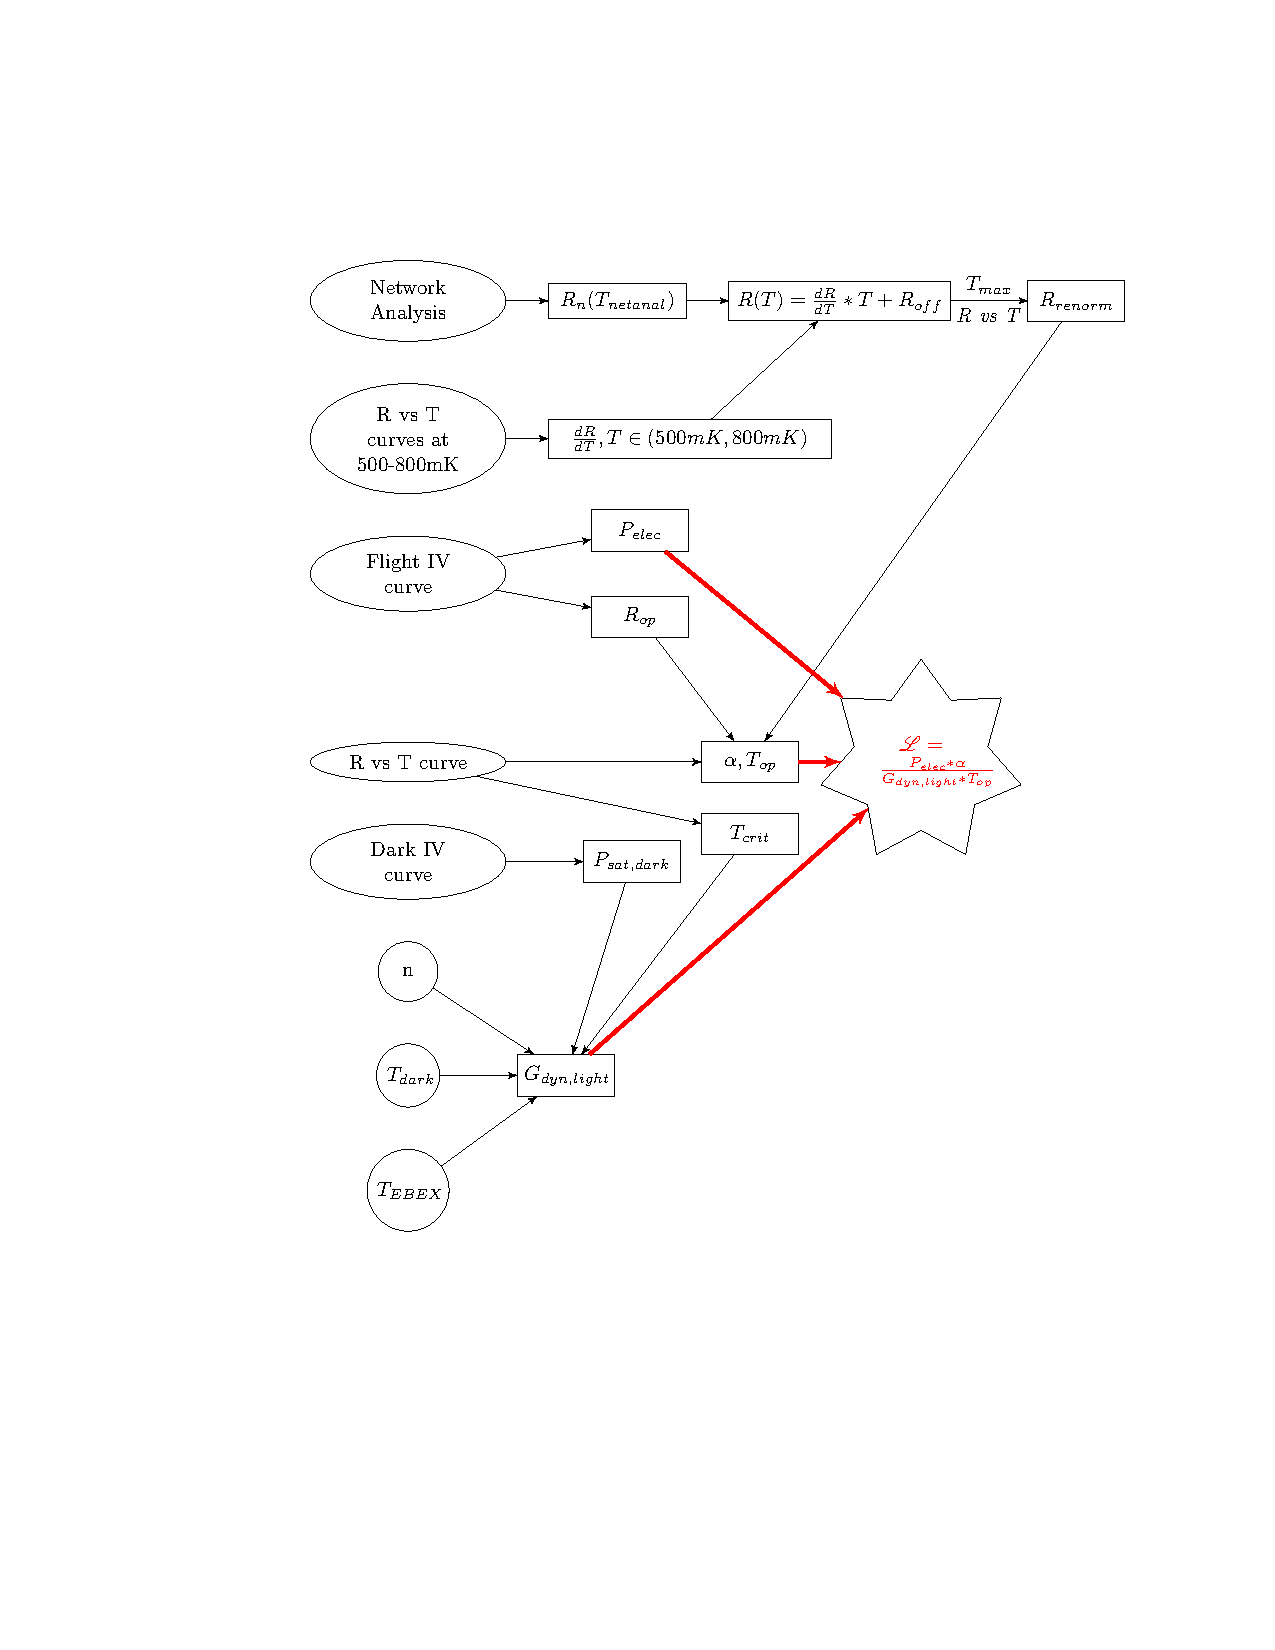
\includegraphics[width=1.0 \textwidth]{figures/loopgain_flowchart.pdf}
\caption{Loop gain calculation flow chart}
\label{fig:loopgain_flow}
\end{center}
\end{figure}

The slope of the Resistance vs Temperature curve for 410-18 between .550 and .800~K was $0.29\pm0.05 \Omega/K$. 

\begin{figure}[htbp]
\begin{center}
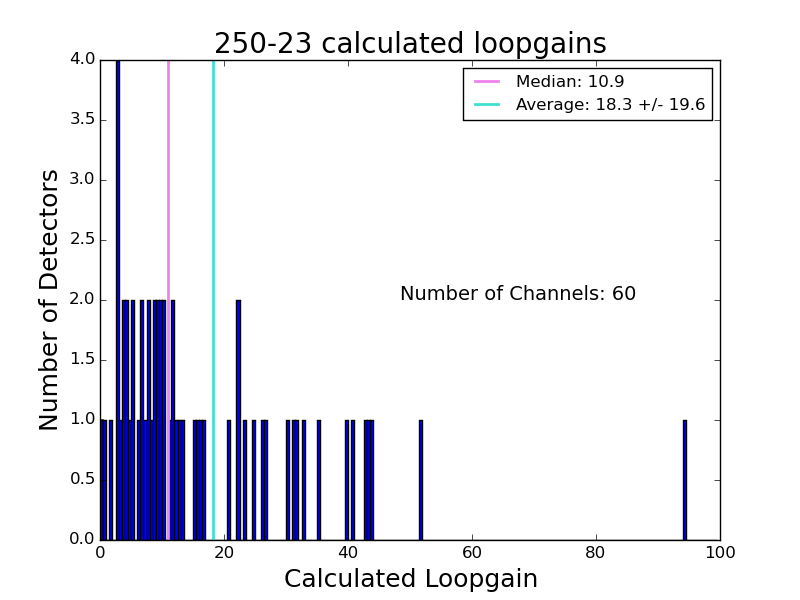
\includegraphics[width=0.5 \textwidth]{figures/250-23_loopgains_calculated_tuning3.png}
\caption{Loop gains calculated for 250-23 for tuning3.}
\label{fig:loopgain_calc_hist}
\end{center}
\end{figure}

\begin{figure}[htbp]
\begin{center}
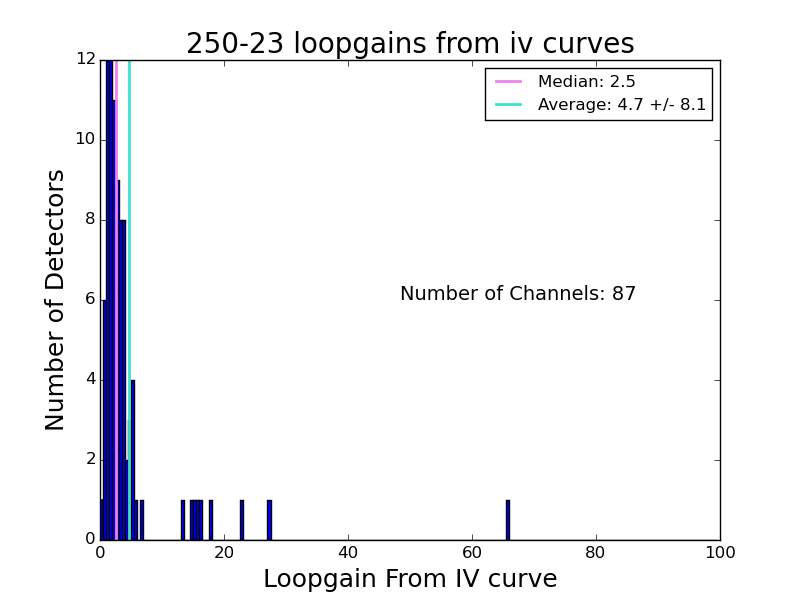
\includegraphics[width=0.5 \textwidth]{figures/250-23_loopgains_from_iv_tuning3.png}
\caption{Loop gains estimated from each 250-23 bolometer's flight IV curve for tuning3.}
\label{fig:loopgain_from_iv_hist}
\end{center}
\end{figure}


%%%%%%%%%%%%%%%%%%%%%%%%%%%%%%%%%%%%%%%%%%%%%%%%%%%%%%%%%%%%%%%%%%%%%%%%%%%%%}}}



%%%%%%%%%%%%%%%%%%%%%%%%%%%%%%%%%%%%%%%%%%%%%%%%%%%%%%%%%%%%%%%%%%%%%%%%%%%%%%%%
% Detector Sensitivity {{{
%%%%%%%%%%%%%%%%%%%%%%%%%%%%%%%%%%%%%%%%%%%%%%%%%%%%%%%%%%%%%%%%%%%%%%%%%%%%%%%%
\section{Detector Sensitivity}
\label{sensitivity}
%%%%%%%%%%%%%%%%%%%%%%%%%%%%%%%%%%%%%%%%%%%%%%%%%%%%%%%%%%%%%%%%%%%%%%%%%%%%%%%%

There are four units we use when measuring the detector noise equivalent power: ADC counts, Amps, Watts at the detector, and Watts on the sky. The total detector noise is recorded in ADC counts by the DfMUX boards. The predictions for the contributions of the current noise terms (Johnson and Readout) are naturally in units of Amps and the predictions for the contributions of the power noise terms (photon and phonon) are naturally in units of Watts at the detector. We also use each detector's calibration map of RCW38 to get a conversion from ADC counts to power on the sky in Watts.

\begin{longtable}{| l | l | l |}
\caption{Noise Equivalent Power, Unit Conversions} \label{NEP_table} \\
  \hline
  Measured Noise & Photon and Phonon Noise & Johnson and Readout Noise \\ \hline
  $\big( \frac{\textbf{cts}^2}{\textbf{Hz}} \big)$ & $\big( \frac{W^2}{Hz} \big) \times \big( \frac{\text{cts}}{A_{sq}} \big) ^2 \times \big( S_I \big) ^2$ & $\big( \frac{A^2}{Hz} \big) \times \big( \frac{\text{cts}}{A_{sq}} \big) ^2 $ \\ \hline
  $\big( \frac{\text{cts}^2}{\text{Hz}} \big) \times \big( \frac{A_{sq}}{\text{cts}} \big) ^2 $ & $\big( \frac{W^2}{Hz} \big) \times \big( S_I \big) ^2$ & $\big( \frac{\textbf{A}^2}{\textbf{Hz}} \big)$ \\ \hline
  $\big( \frac{\text{cts}^2}{\text{Hz}} \big) \times \big( \frac{A_{sq}}{\text{cts}} \big) ^2 \times \big( \frac{1}{S_I} \big) ^2$ & $\big( \frac{\textbf{W}^2}{\textbf{Hz}} \big)$ & $\big( \frac{A^2}{Hz} \big) \times \big( \frac{1}{S_I} \big) ^2$ \\ \hline
  $\big( \frac{\text{cts}^2}{\text{Hz}} \big) \times \big( \frac{W_{sky}}{\textbf{cts}} \big) ^2$ & $\big( \frac{W^2}{Hz} \big) \times \big( \frac{1}{\varepsilon} \big) ^2$ & $\big( \frac{A^2}{Hz} \big) \times \big( \frac{\text{cts}}{A_{sq}} \big) ^2 \times \big( \frac{W_{sky}}{\text{cts}} \big) ^2$ \\ \hline
\end{longtable}

$\varepsilon$ is the instrument efficiency.
\be
\varepsilon = \frac{\text{power absorbed by detector}}{\text{incident sky power}}
\label{eq:eff_ratio}
\ee

Responsivity is
\be
S_I = \frac{-1}{V_{bias}} * \frac{\mathscr{L}}{\mathscr{L} + 1} * \frac{1}{1 + i\omega\tau}
\label{eq:current_responsivity}
\ee

In the normal region of the resistance versus temperature curve, \ac{EBEX} wafer 410-18 detectors have an average slope $dR/dT$ of $0.29\pm0.05 \Omega/K$. 
At the transition temperature, the average slope of the curve is found to be XXX $\Omega/K$, a factor of XXX greater. 
The loopgain is proportional to $dR/dT$ and so it is a factor of $\sim XXX$ smaller when the detector is overbiased. 
The factor $\mathcal{L}/(\mathcal{L}+1)$ is XXX when the detector is normal versus XXX when the detector is overbiased. 
The dominant noise contributions are then from the Johnson and readout noise. 

%%%%%%%%%%%%%%%%%%%%%%%%%%%%%%%%%%%%%%%%%%%%%%%%%%%%%%%%%%%%%%%%%%%%%%%%%%%%%}}}


%%%%%%%%%%%%%%%%%%%%%%%%%%%%%%%%%%%%%%%%%%%%%%%%%%%%%%%%%%%%%%%%%%%%%%%%%%%%%%%%
% Flight Noise Performance {{{
%%%%%%%%%%%%%%%%%%%%%%%%%%%%%%%%%%%%%%%%%%%%%%%%%%%%%%%%%%%%%%%%%%%%%%%%%%%%%%%%
\section{Flight Noise Performance}
\label{flight_noise_performance}
%%%%%%%%%%%%%%%%%%%%%%%%%%%%%%%%%%%%%%%%%%%%%%%%%%%%%%%%%%%%%%%%%%%%%%%%%%%%%%%%

The following analysis looks at the 941 bolometers wired to \ac{BRO}s 2, 3, and 4. 
With the exception of the very first time the bolometers were dropped into their transitions at float and the subsequent half hour of observation, \ac{BRO}1 was turned off in order to conserve bolometer power. \ac{BRO}1 also happened to consist of wafers which were largely saturated at float. 
Of the 941 bolometers included, 303 of them have zero valid samples throughout flight. 
An additional 92 bolometers have no 172~second chunks without flags. 
That should leave us with 546 detectors with some good data. 
There are, however, only 398 detectors reported in the analysis. 
We have 148 unaccounted for detector losses. 



noise at float blah blah blah

\begin{figure}[ht]
\centering
   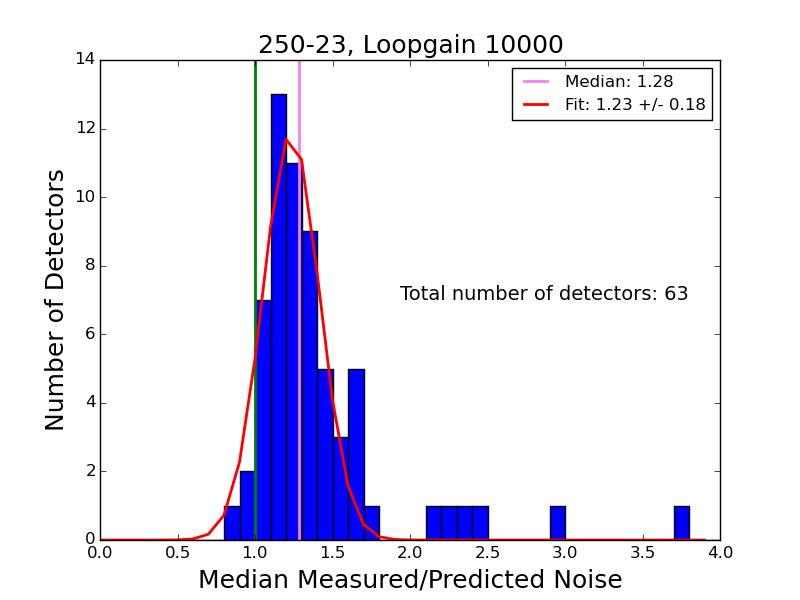
\includegraphics[width=0.33\textwidth]{./figures/250-23_it_meas_pred_ratio_loopgain_10000.png}
   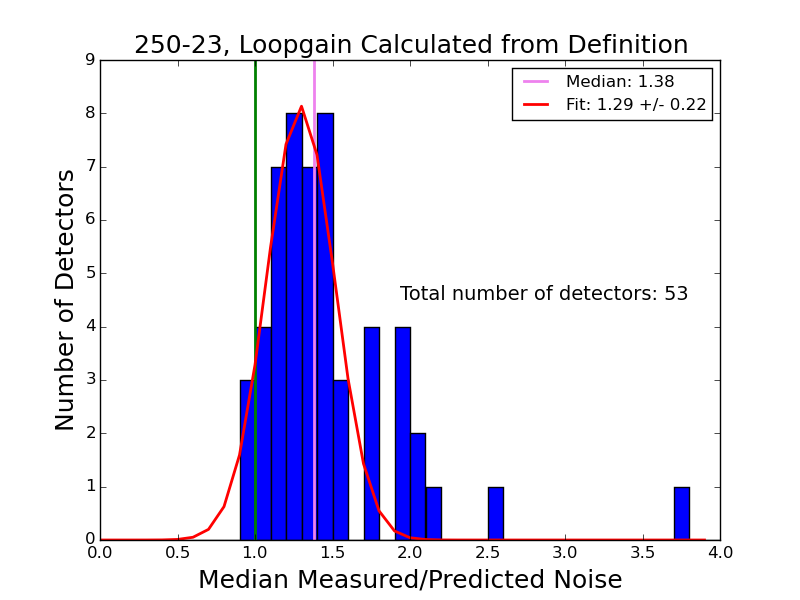
\includegraphics[width=0.33\textwidth]{./figures/250-23_it_meas_pred_ratio_loopgain_calc.png}
   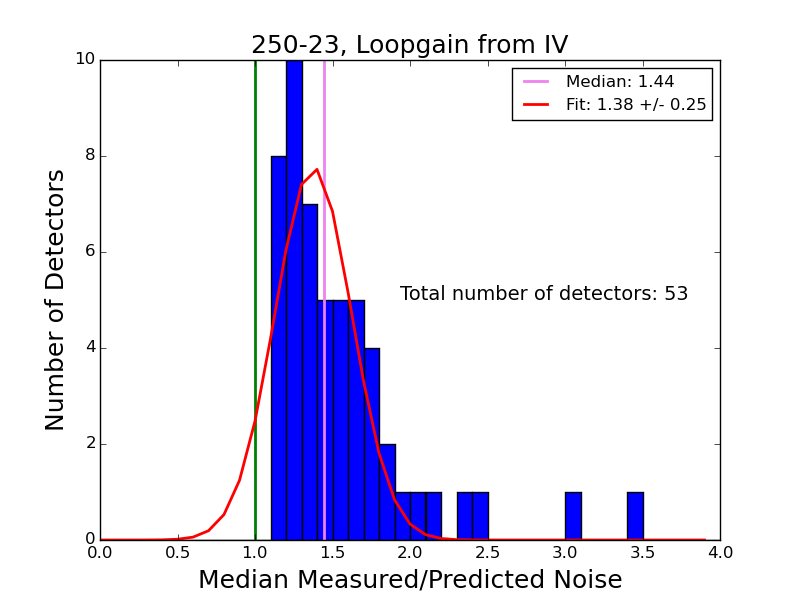
\includegraphics[width=0.33\textwidth]{./figures/250-23_it_meas_pred_ratio_loopgain_iv.png}
\caption{Wafer 250-23 noise performance for three different loopgain value scenarios. The most optimistic is to assume the detectors are
                deep in the transition (NEED TO DEFINE THIS) and so the loopgain is huge, $L$=10000 (upper left). If the detectors are not 
                deep in the transition, we can calculate the loopgain and include it in the conversion from counts to power. The loopgain 
                can be calculated from its definition (upper right) and can also be estimated from the IV curve (lower).  
                \label{fig:effect_of_loopgain}}
\end{figure}


%%%%%%%%%%%%%%%%%%%%%%%%%%%%%%%%%%%%%%%%%%%%%%%%%%%%%%%%%%%%%%%%%%%%%%%%%%%%%}}}
